% Section 5: Overfitting and Generalization (Slides 33-39)

% Slide 33: Practical Issue: Overfitting - Tree 1
\begin{frame}{مسئله بیش‌برازش در عمل: درخت اول}{\lr{Practical Issue: Overfitting (Tree 1)}}
  \begin{columns}[c]
    \begin{column}{0.62\textwidth}
      \begin{itemize}
        \item \textbf{نمونه کاربردی:} پیش‌بینی رتبه اعتباری مشتریان (\lr{Credit Rating})
        \item یک ساختار درخت تصمیم ممکن:
      \end{itemize}
    \end{column}
    \begin{column}{0.36\textwidth}
      \centering
      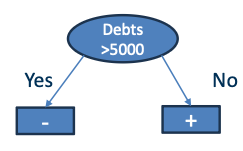
\includegraphics[width=\textwidth,height=2.2cm,keepaspectratio]{images/slide33_tree1_clean.png}
    \end{column}
  \end{columns}
  \vspace{0.1cm}
  \begin{center}
    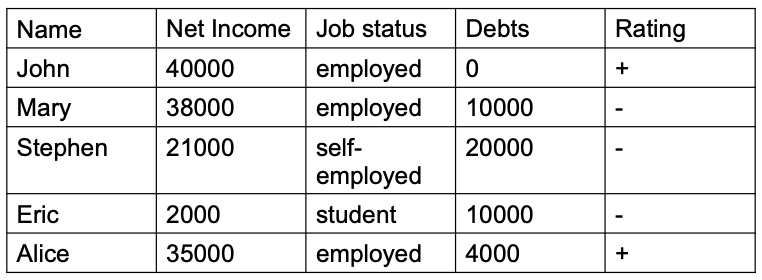
\includegraphics[width=0.85\textwidth,height=2.6cm,keepaspectratio]{images/slide33_table_clean.png}
  \end{center}
\end{frame}

% Slide 34: Practical Issue: Overfitting - Tree 2
\begin{frame}{مسئله بیش‌برازش در عمل: درخت دوم}{\lr{Practical Issue: Overfitting (Tree 2)}}
  \begin{columns}[c]
    \begin{column}{0.62\textwidth}
      \begin{itemize}
        \item \textbf{همان مسئله}، اما با ساختار جایگزین و شاخه‌بندی بر اساس نام افراد:
      \end{itemize}
    \end{column}
    \begin{column}{0.36\textwidth}
      \centering
      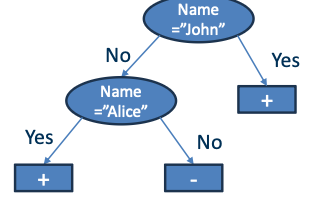
\includegraphics[width=\textwidth,height=2.3cm,keepaspectratio]{images/slide34_tree2_clean.png}
    \end{column}
  \end{columns}
  \vspace{0.1cm}
  \begin{center}
    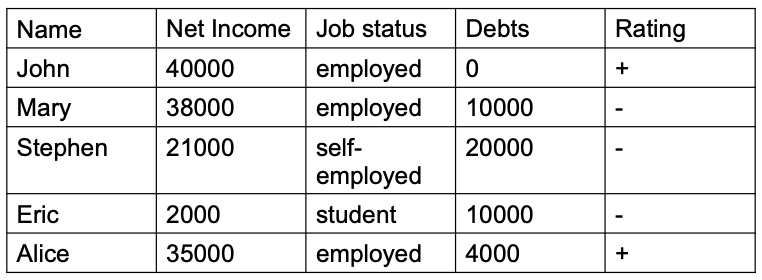
\includegraphics[width=0.85\textwidth,height=2.6cm,keepaspectratio]{images/slide33_table_clean.png}
  \end{center}
\end{frame}

% Slide 35: Overfitting: Comparison
\begin{frame}{مسئله بیش‌برازش در عمل: مقایسه دو درخت}{\lr{Practical Issue: Overfitting}}
  \begin{itemize}
    \setlength{\itemsep}{3pt}
    \item \textbf{هر دو درخت به یک اندازه خوب به نظر می‌رسند:}
    \begin{itemize}
      \item تمام نمونه‌های آموزش را با دقت کامل و صحت \lr{100\%} طبقه‌بندی می‌کنند.
    \end{itemize}
    \item \textbf{شما کدام درخت را ترجیح می‌دهید؟}
  \end{itemize}
  \vspace{0.15cm}
  \begin{center}
    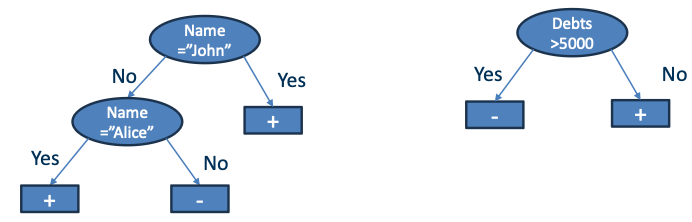
\includegraphics[width=0.90\textwidth,height=3.8cm,keepaspectratio]{images/slide35_credit_comparison_clean.png}
  \end{center}
\end{frame}

% Slide 36: Occam's Razor
\begin{frame}{تیغ اوکام}{\lr{Occam's Razor}}
  \begin{columns}[T]
    \begin{column}{0.65\textwidth}
      \begin{itemize}
        \setlength{\itemsep}{8pt}
        \item \textbf{پیشینه:} منسوب به \textbf{ویلیام اوکام (\lr{William of Ockham}، ۱۲۸۷--۱۳۴۷)}، فیلسوف نامی سده‌های میانه.
        \item \textbf{قاعده اصیل:} «تعداد موجودات نباید فراتر از ضرورت افزایش یابد».
        \item \textbf{کاربرد در یادگیری ماشین:}
        \begin{itemize}
          \item «در میان مدل‌هایی که دقت برابری دارند، همواره ساده‌ترین مدل ارجح است».
          \item درختی با ساختار کم‌عمق‌تر و شاخه‌های کمتر، شانس بسیار بالاتری برای تعمیم به داده‌های نادیده دارد.
        \end{itemize}
      \end{itemize}
    \end{column}
    \begin{column}{0.32\textwidth}
      \begin{center}
        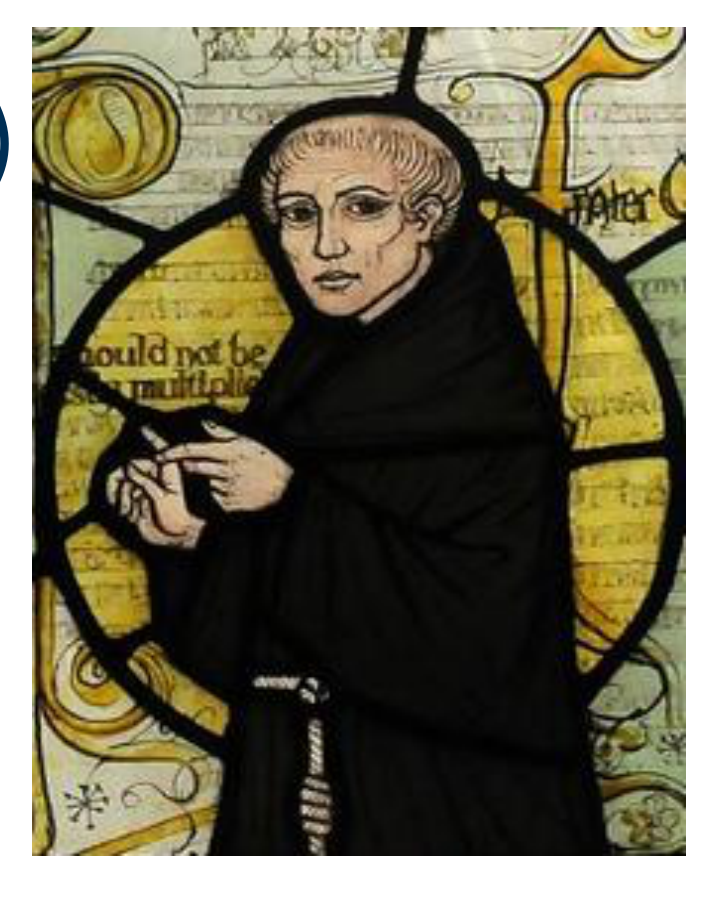
\includegraphics[width=0.85\textwidth,height=4.0cm,keepaspectratio]{images/slide36_occam_portrait.png}\\[0.1cm]
        {\scriptsize\color{subgray}ویلیام اوکام (۱۲۸۷--۱۳۴۷)}
      \end{center}
    \end{column}
  \end{columns}
\end{frame}

% Slide 37: Training and Testing Data
\begin{frame}{جداسازی داده‌های آموزش و آزمون}{\lr{Training and Testing Data}}
  \begin{columns}[T]
    \begin{column}{0.54\textwidth}
      \begin{itemize}
        \setlength{\itemsep}{7pt}
        \item \textbf{خطای آموزش فریبنده است:} ارزیابی مدل با همان داده‌هایی که در آموزش استفاده شده‌اند، منجر به برآوردی به شدت خوش‌بینانه و نادرست می‌شود.
        \item \textbf{لزوم تفکیک مستقل:} ارزیابی واقعی عملکرد تعمیم (\lr{Generalization}) تنها با اعمال مدل بر روی داده‌های آزمون مجزا که مدل هرگز ندیده است امکان‌پذیر است.
      \end{itemize}
    \end{column}
    \begin{column}{0.44\textwidth}
      \begin{center}
        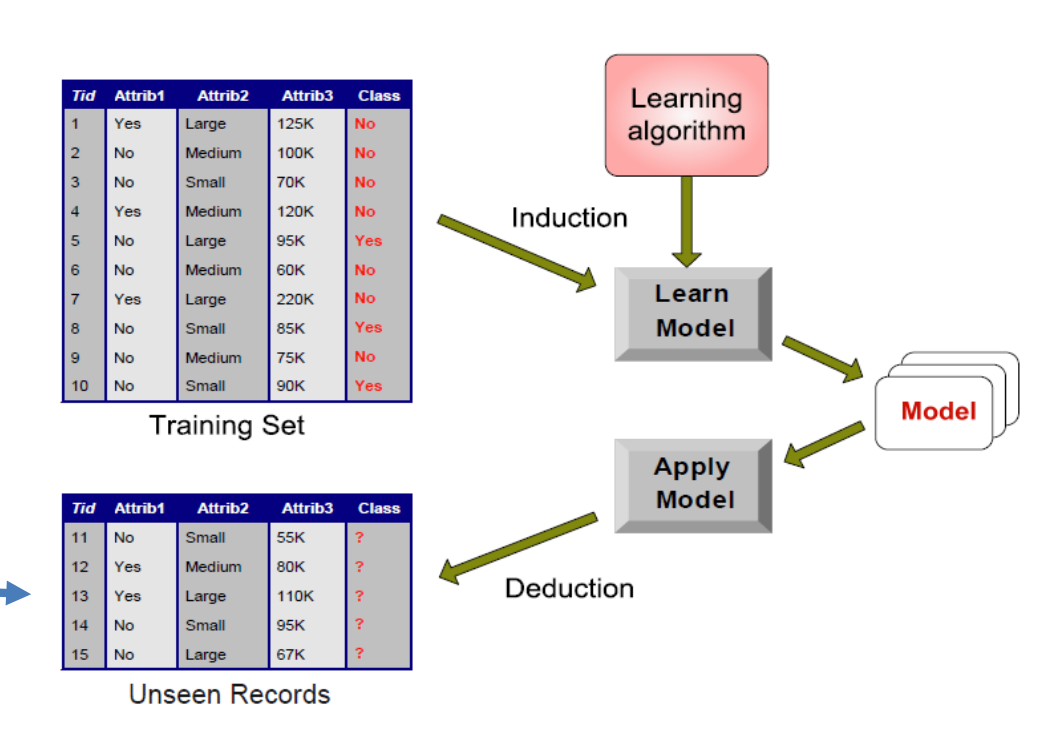
\includegraphics[width=\textwidth,height=5.0cm,keepaspectratio]{images/slide37_workflow_test.png}
      \end{center}
    \end{column}
  \end{columns}
\end{frame}

% Slide 38: Overfitting: Symptoms and Causes
\begin{frame}{بیش‌برازش: نشانه‌ها و علل}{\lr{Overfitting: Symptoms and Causes}}
  \begin{columns}[T]
    \begin{column}{0.50\textwidth}
      \begin{itemize}
        \setlength{\itemsep}{5pt}
        \item \textbf{نشانه‌ها:} \lr{(Symptoms)}
        \begin{itemize}
          \item عمق بیش از حد درخت و شاخه‌بندی‌های ریز
          \item خطای نزدیک به صفر در آموزش ولی خطای بالا در آزمون
        \end{itemize}
        \item \textbf{علل اصلی:} \lr{(Causes)}
        \begin{itemize}
          \item وجود نویز و داده‌های پرت در مجموعه آموزش
          \item تعداد اندک نمونه‌های آموزشی نسبت به پیچیدگی فضا
        \end{itemize}
      \end{itemize}
    \end{column}
    \begin{column}{0.48\textwidth}
      \begin{center}
        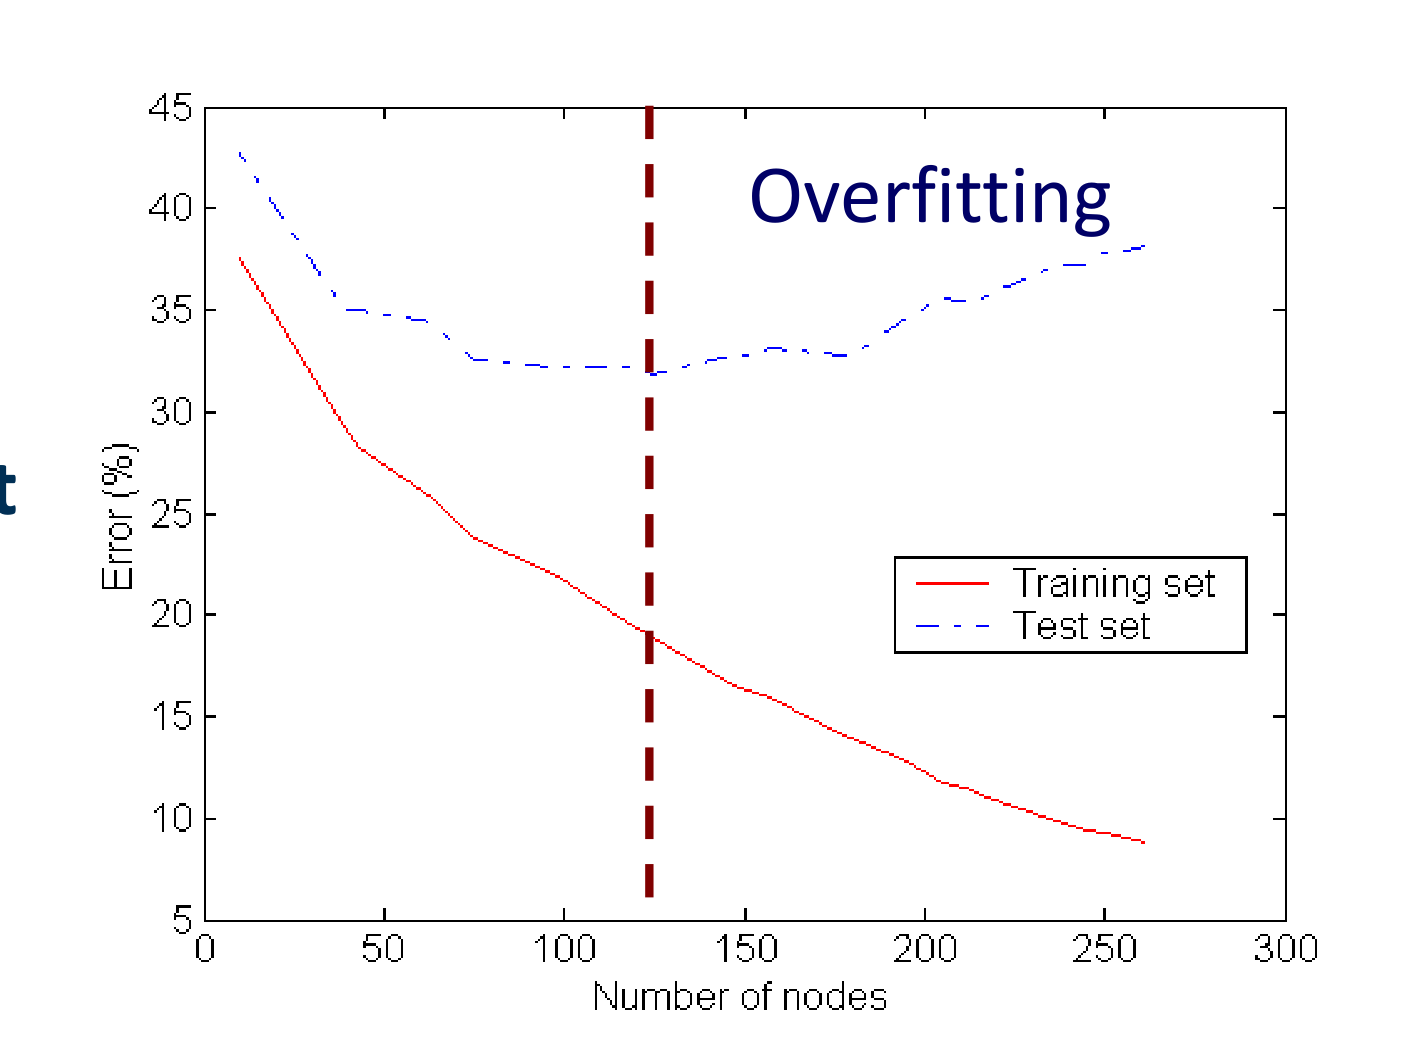
\includegraphics[width=\textwidth,height=4.8cm,keepaspectratio]{images/slide38_overfitting_curve.png}
      \end{center}
    \end{column}
  \end{columns}
\end{frame}

% Slide 39: Overfitting and Noise
\begin{frame}{بیش‌برازش و نویز داده‌ها}{\lr{Overfitting and Noise}}
  \begin{itemize}
    \item انطباق وسواسی مرزهای تصمیم بر روی نمونه‌های منفرد نویز موجب تخریب مرز واقعی کلاس‌ها می‌شود:
  \end{itemize}
  \vspace{0.1cm}
  \begin{columns}[T]
    \begin{column}{0.48\textwidth}
      \begin{center}
        \textbf{\footnotesize مدل بیش‌برازش‌شده (برازش نویز)}\\[0.05cm]
        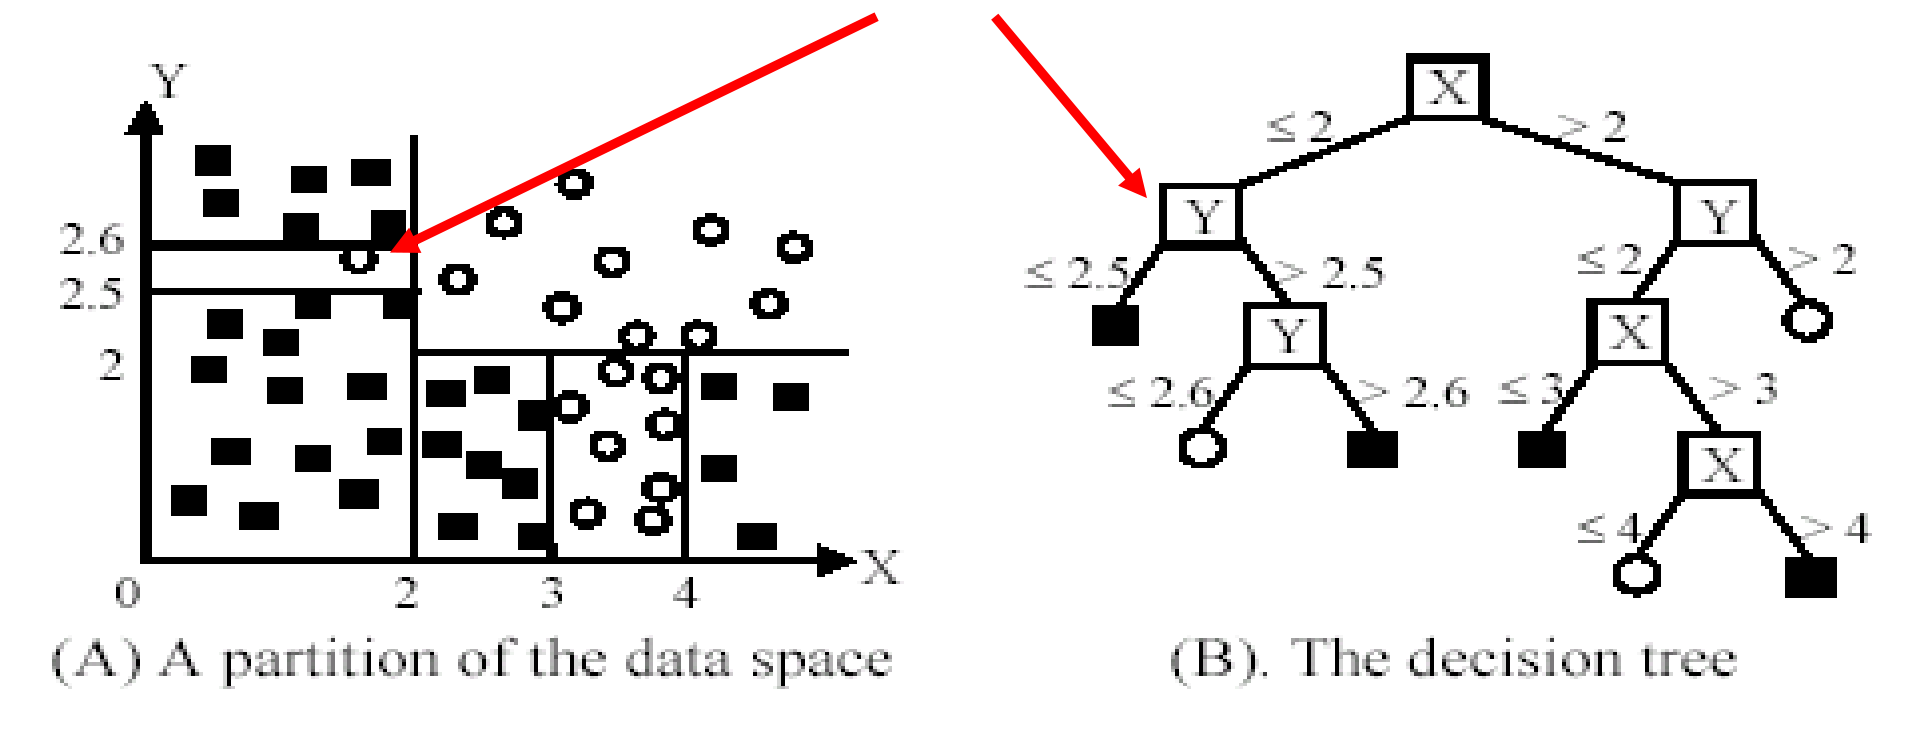
\includegraphics[width=\textwidth,height=3.4cm,keepaspectratio]{images/slide39_noise_overfit.png}
      \end{center}
    \end{column}
    \begin{column}{0.48\textwidth}
      \begin{center}
        \textbf{\footnotesize مدل ساده‌تر (تعمیم‌پذیری بالا)}\\[0.05cm]
        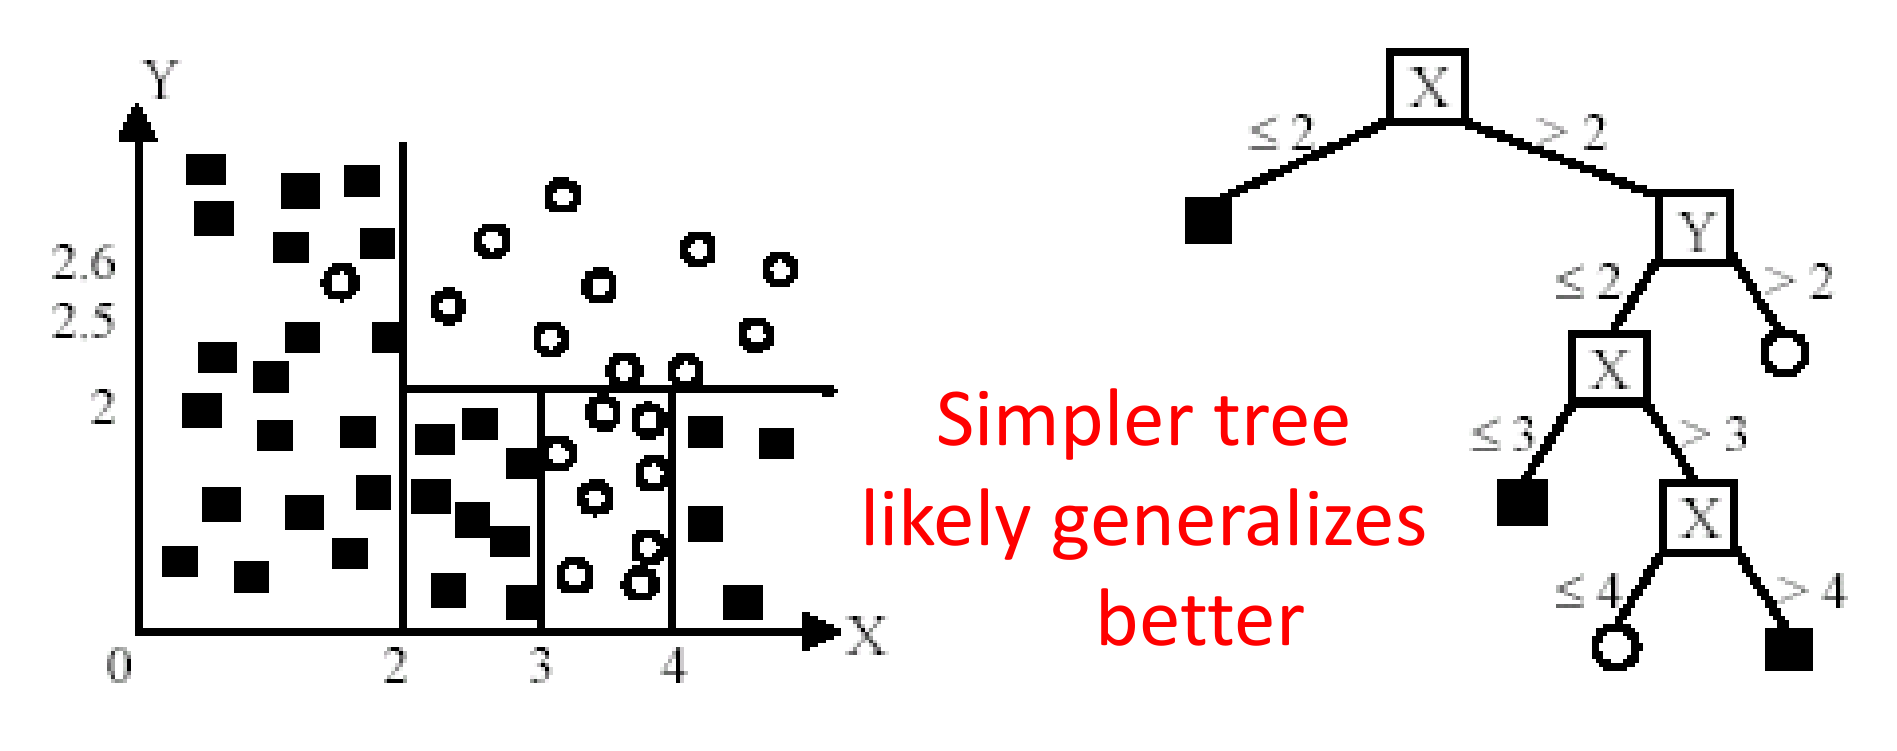
\includegraphics[width=\textwidth,height=3.4cm,keepaspectratio]{images/slide39_noise_simpler.png}
      \end{center}
    \end{column}
  \end{columns}
\end{frame}
